\documentclass[crop,tikz]{standalone}

\usetikzlibrary{calc,patterns,angles,quotes}

\begin{document}

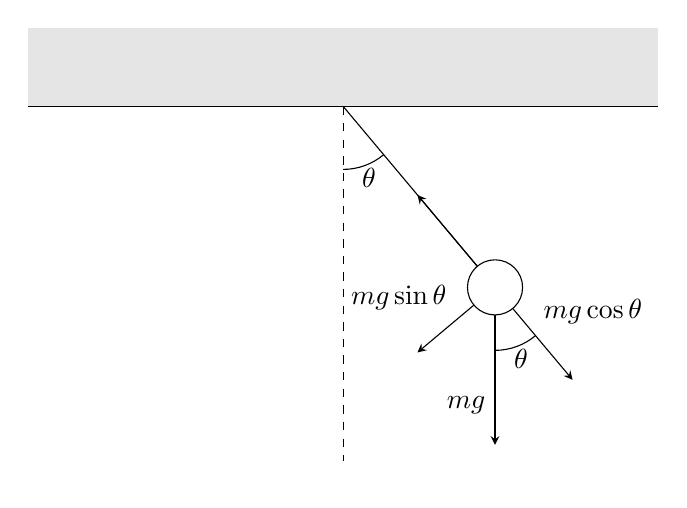
\begin{tikzpicture}
	% Techo
	\fill[color=gray!20] (-4,1) rectangle (4,0);
	\draw (-4,0) -- (4,0);

    % save length of g-vector and theta to macros
    \pgfmathsetmacro{\Gvec}{2}
    \pgfmathsetmacro{\angulo}{40}
    % calculate lengths of vector components
    \pgfmathsetmacro{\Gcos}{\Gvec*cos(\angulo)}
    \pgfmathsetmacro{\Gsin}{\Gvec*sin(\angulo)}

	% anclaje al techo
    \coordinate (anclaje) at (0,0);

	% normal al techo
    \draw[dashed] (anclaje) -- ++(0,-4.5) node (normal) [black,below]{$ $};

	% cuerda
    \draw (anclaje) -- ++(270+\angulo:3) coordinate (centro);

	% ángulo theta cerca del techo
    \pic [draw, "$\theta$", angle eccentricity=1.2, angle radius=.8cm] 
		{angle = normal--anclaje--centro};


    \draw [-stealth] (centro) -- ($(centro)!\Gcos cm!(anclaje)$);
    \draw [-stealth] (centro) -- ($(centro)!-\Gcos cm!(anclaje)$)
      coordinate (gcos)
      node[midway,above right] {$mg\cos\theta$};
    \draw [-stealth] (centro) -- ($(centro)!\Gsin cm!90:(anclaje)$)
      coordinate (gsin)
      node[midway,above left] {$mg\sin\theta$};
    \draw [-stealth] (centro) -- ++(0,-\Gvec)
      coordinate (g)
      node[near end,left] {$mg$};

	% ángulo theta bajo la bola
    \pic [draw, "$\theta$", angle eccentricity=1.2, angle radius=.8cm] 
		{angle = g--centro--gcos};

	% bola
    \filldraw [fill=white,draw=black] (centro) circle[radius=.35];
\end{tikzpicture}

\end{document}
